\chapter{احتمال شرطی در متغیرهای تصادفی}

\Q
اگر متغیر تصادفی 
$
X
$
را دارای چگالی احتمال زیر در نظر بگیریم
\eqn{
f_X(x)=\begin{cases}
{1\over 2}&,\quad 0<x<2\\
0&,\quad \text{سایر جاها}
\end{cases}
}
موارد 
$
F(x|X<1)
$
(توزیع تجمعی)
،
$
f(x|X>1)
$
(چگالی احتمال)
و
$
\mathbb{E}\{X|0.5<X<1.5\}
$
را بیابید.

%%%%%%%%%%%%%%%%%%%%%%%%%%%%%%%%%%%%%%

\Q
فرض کنید متغیر تصادفی 
$
X
$
 دارای چگالی احتمال زیر باشد
\eqn{
f_X(x)=
\begin{cases}
\lambda e^{-\lambda x} &,\quad x>0\\
0&,\quad \text{سایر جاها}
\end{cases} \quad,\quad \lambda>0
}
در این صورت مقادیر 
$
\mathbb{E}\{X|X>a\}
$
و
$
\mathbb{E}\{X\}+a
$
را بیابید و با هم مقایسه کنید. نتیجه را تفسیر کنید و ببینید آیا با شهود سازگار است. این چه ویژگی ای از متغیرهای تصادفی نمایی را نشان می دهد؟

%%%%%%%%%%%%%%%%%%%%%%%%%%%%%%%%%%%%%%

\Q
برای متغیر تصادفی 
$X$
با توزیع زیر
\eqn{
\Pr\{X=i\}=(1-p)^i\cdot p\quad,\quad i=0,1,2,\cdots
}
الف) مقدار 
$\text{var}\{X|X\ge 4\}$
را به دست آورید.

ب) تابع جرم احتمال شرطی 
$\Pr\{X=x|\text{X زوج است}\}$
را پیدا کنید.

%%%%%%%%%%%%%%%%%%%%%%%%%%%%%%%%%%%%%%

\Q
تاس سالمی را 9 بار پرتاب می‌کنیم. اگر متغیر تصادفی $X$، تعداد اعداد زوج رو آمده به شرط دانستن این باشد که در سه پرتاب اول، حداقل یک عدد فرد آمده است،

الف)  چگالی احتمال $X$ را محاسبه کنید.

ب) اگر متغیر تصادفی $Y$، تعداد اعداد اول رو آمده باشد، مقدار 
$\Pr\{X=x|Y=0\}$
 چقدر است؟

%%%%%%%%%%%%%%%%%%%%%%%%%%%%%%%%%%%%%%

\Q
سکه ای را 10 بار پرتاب می کنیم. متغیر تصادفی $X$ برابر تعداد دفعات رو آمدن در پرتاب های دوم و چهارم و متغیر تصادفی $Y$ برابر تعداد دفعات پشت آمدن در 2 پرتاب اول است. مقدار 
$\mathbb{E}\{XY\}$
و چگالی احتمال شرطی
$f_{X|Y}(X=x|Y=y)$
 را به دست آورید (می توانید از روش جدول نویسی برای چگالی احتمال استفاده کنید که سطر جدول $X=x$ و ستون جدول $Y=y$ است).

%%%%%%%%%%%%%%%%%%%%%%%%%%%%%%%%%%%%%%

\Q
 در پرتاب 10 بار سکه‌ی سالم به طور مستقل،

الف) توزیع احتمال متغیر تصادفی تعداد سکه های شیر آمده را به شرط آن که بدانیم سه پرتاب اول خط بوده اند به دست آورید.

ب) توزیع احتمال متغیر تصادفی تعداد سکه های شیر آمده را به شرط آن که بدانیم دست کم دو پرتاب از سه پرتاب اول خط بوده اند به دست آورید.

%%%%%%%%%%%%%%%%%%%%%%%%%%%%%%%%%%%%%%

\Q
کانال مخابراتی زیر را در نظر بگیرید:

\begin{figure}[h]
\centering
\Large
\lr{
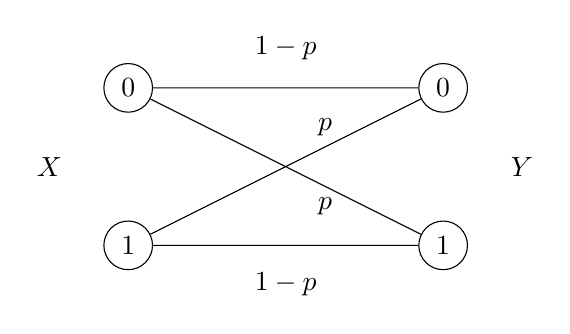
\begin{tikzpicture}
\node [draw=black,circle] (1) at(0,0) {0};
\node [draw=black,circle] (2) at(4,0) {0};
\node [draw=black,circle] (3) at(0,-2) {1};
\node [draw=black,circle] (4) at(4,-2) {1};
\draw 
(1) -- (2)
(1) -- (4)
(3) -- (2)
(3) -- (4)
;
\node (5) at(2,0.5) {$1-p$};
\node (6) at(2.5,-0.5) {$p$};
\node (7) at(2.5,-1.5) {$p$};
\node (8) at(2,-2.5) {$1-p$};
\node (9) at(-1,-1) {$X$};
\node (10) at(5,-1) {$Y$};
\end{tikzpicture}
}
\end{figure}

که در آن، پیکان ها احتمالات گذار را از متغیر تصادفی $X$ به متغیر تصادفی $Y$ نشان می دهند؛ به طور مثال
$
\Pr\{Y=0|X=1\}=p
$.

الف) اگر 
$
\Pr\{X=0\}=q
$
 که 
$
0\le q\le 1
$
، در اینصورت توزیع توام $X$ و $Y$ را محاسبه کنید.

ب) احتمال خطا (
$
\Pr\{X\ne Y\}
$
)
 را محاسبه کنید. اگر مقدار $p$ ثابت باشد، آیا احتمال خطا بر حسب $q$ نقطه‌ی بهینه دارد؟ اگر دارد آنرا بیابید و در غیر این صورت، علت را بیان کنید.

\Q
اگر توزیع تجمعی یک متغیر تصادفی ترکیبی به صورت 
$$
F(x)=\begin{cases}
0&,\quad x<0\\
{x+2\over 4}&,\quad 0\le x<1\\
1&,\quad x\ge 1
\end{cases}
$$
باشد، چگالی احتمال متغیر تصادفی 
$
X|(X\ne 0\text{\rl{ یا }}X\ne 1)
$
 را به دست آورید.


\Q
اگر برای متغیرهای تصادفی $X$ و $Y$، چگالی احتمال زیر را داشته باشیم
$$
f_{XY}(x,y)=\begin{cases}e^{-x(y+1)^2}&,\quad x,y>0\\
0&,\quad \text{\rl{در غیر این صورت}}\end{cases}
$$
در این صورت توزیع $X|Y=y$ را به دست آورید.

\Q
فرض کنید متغیر تصادفی $X$، نتیجه پرتاب یک تاس سالم باشد. سپس با توجه به رخداد 
$X$
، متغیر تصادفی پیوسته‌ی
$Y$
را به صورت شرطی با چگالی احتمال زیر تعریف می‌کنیم:
\eqn{
f_{Y|X}(x,y)=\begin{cases}
{1\over x}&,\quad 0<y<x\\
0&,\quad \text{سایر جاها}
\end{cases}
}

الف) احتمال 
$\Pr\{Y\ge 3\}$
را بیابید.

ب) چگالی احتمال 
$f_Y(y)$
را به دست آورید.

پ) مقادیر 
$\mathbb{E}\{Y\}$
و
$\text{var}(Y)$
را از روی چگالی احتمال $Y$ محاسبه کنید.



\Q
برای چگالی احتمال زیر، مقادیر
$
\mathbb{E}\{X|X>1\}
$
و
$
\sigma_X^2(X|X>1)
$
و چگالی های احتمال شرطی
$
f(x|X\ne 1)
$
و
$
f(x|X<\frac{1}{2})
$
 را محاسبه کنید.
$$
f_X(x)=\begin{cases}
3x(1-x)&,\quad 0<x<1\\
\frac{1}{2}\delta(x-1)&,\quad x=1\\
0&,\quad \text{سایر جاها}
\end{cases}
$$

\Q
چگالی احتمال توأم زیر برای دو متغیر تصادفی $X$ و $Y$ داده شده است:
$$
f_{X,Y}(x,y)=\begin{cases}
\frac{1}{\pi}&,\quad x^2+y^2\le 1\\
0&,\quad \text{سایر جاها}
\end{cases}
$$

الف) چگالی احتمال شرطی
$
f_{\max\{X,Y\}}(u|X\le \frac{1}{2})
$
را بیابید (ابتدا 
$
\Pr\{\max\{X,Y\}\le u|X\le \frac{1}{2}\}
$
را محاسبه کنید).

ب) مقدار 
$
\mathbb{E}\{\sqrt{X^2+Y^2}|X+Y\le 1\}
$
را بیابید.

\Q
اطلاعات زیر در مورد دو متغیر تصادفی $X$ و $Y$ داده شده است:
\eqn{
&\Pr\{X=-1\}=\Pr\{X=1\}=\frac{1}{2}
\\&
f_Y(y|X=x)=\frac{a}{2}\exp(-a|x-y|)
}
که $a$، عدد ثابت مثبتی است.

الف) احتمال های
$
\Pr\{Y\le 0|X=1\}
$
و
$
\Pr\{Y\ge 0|X=-1\}
$
را بیابید. با افزایش $a$، مقادیر احتمالهای فوق چه تغییر می‌کنند؟

ب) نتیجه‌ی قسمت الف را با دیدگاه احتمال خطا توجیه کنید.